
%!TEX TS-program = lualatex
%!TEX encoding = UTF-8 Unicode

%\frame[plain]{ % When including a large figure or table, you don't want to have the bottom and the top of the slides.
%\frame[shrink]{ % If you want to include lots of text on a slide, use the shrink option.


\begin{frame}[plain]
    \frametitle{Throughput Relative to Linux Loopback Mounting}
    \vspace*{-1pt}
    \makebox[\linewidth]{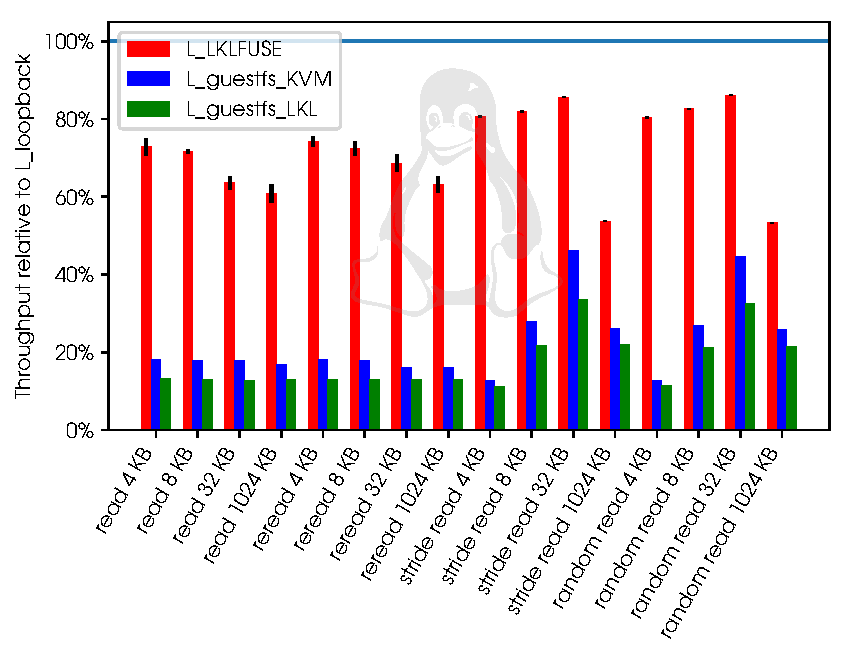
\includegraphics[page=1,width=0.87\paperwidth]{frames/img/relative_performance_filter_read_baseline_L_loopback_variants_L_LKLFUSE_L_guestfs_KVM_L_guestfs_LKL}}
    \note{
        \begin{itemize}
            \item X-axis, workloads, read, reread. stride read, random read
            \item Y-access relative to baseline loopback-mounting
            \item three colors, red LKLFUSE, blue guestfs KVM, green guestfs LKL
            \item LKLFUSE delivers okay read performance, i.e. 72\%
            \item very consistent irregardless of blocksize. readahead
            \item loopback has readahead as well. possible that amplification occurrs over several layers
            \item less pronounced effect for stride and random read
            \item libguestfs is too slow. architecture not made for FUSE but CLI.
            \item mostly caused by the communication protocol overhead.
            \item guestfs-LKL worse than KVM around 80\%. Profiling needed
            \item I expect it to be possible to optimize the prototypic LKL-backend so that it outperforms the LKL-backend

        \end{itemize}
    }
\end{frame}

\begin{frame}[plain]
\frametitle{Throughput Relative to Linux Loopback Mounting}
\vspace*{-1pt}
\makebox[\linewidth]{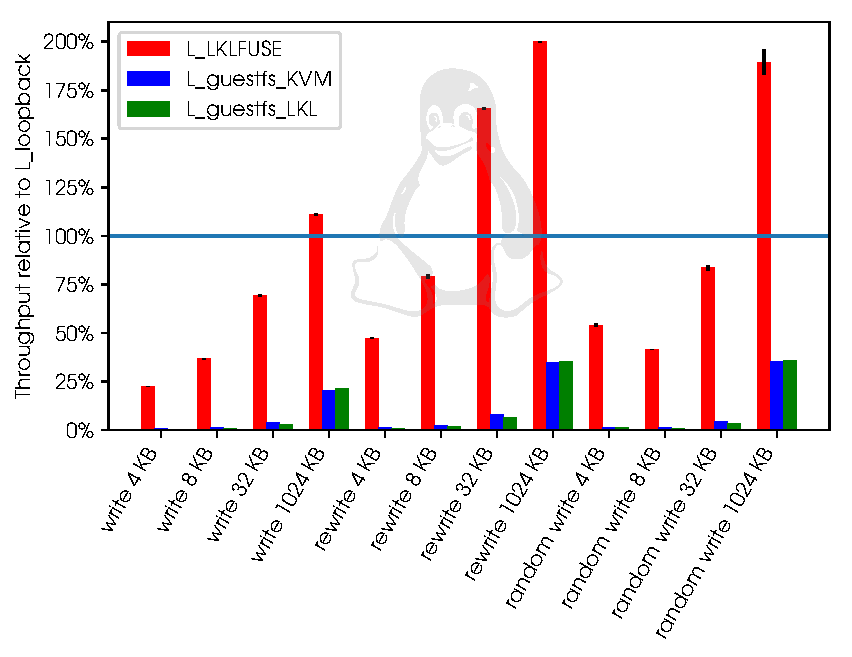
\includegraphics[page=1,width=0.87\paperwidth]{frames/img/relative_performance_filter_write_baseline_L_loopback_variants_L_LKLFUSE_L_guestfs_KVM_L_guestfs_LKL}}
\note{
    \begin{itemize}
        \item LKLFUSE: seq write delivers okay performance, i.e. above 50\%
        \item big difference between blocksizes. Overhead of each write reaching the FS one by one
        \item much better than baseline: how is that possible. No fsync!
        \item writing to pages that have not been written back (rewrite, random write), writeback caching
        \item FUSE does not have it, but the lower layers (LKL and read of image)
        \item many moving parts, two kernels, several caches, readahead...
        \item libguestfs-lkl is too slow
        \item mostly caused by the communication protocol overhead.
        \item libguestfs-kvm is only slightly faster
        \item I expect it to be possible to optimize the prototypic LKL-backend so that it outperforms the LKL-backend
        
    \end{itemize}
}
\end{frame}

\begin{frame}[plain]
    \frametitle{Throughput Relative to Windows VHD Mounting}
    \vspace*{-1pt}
    \makebox[\linewidth]{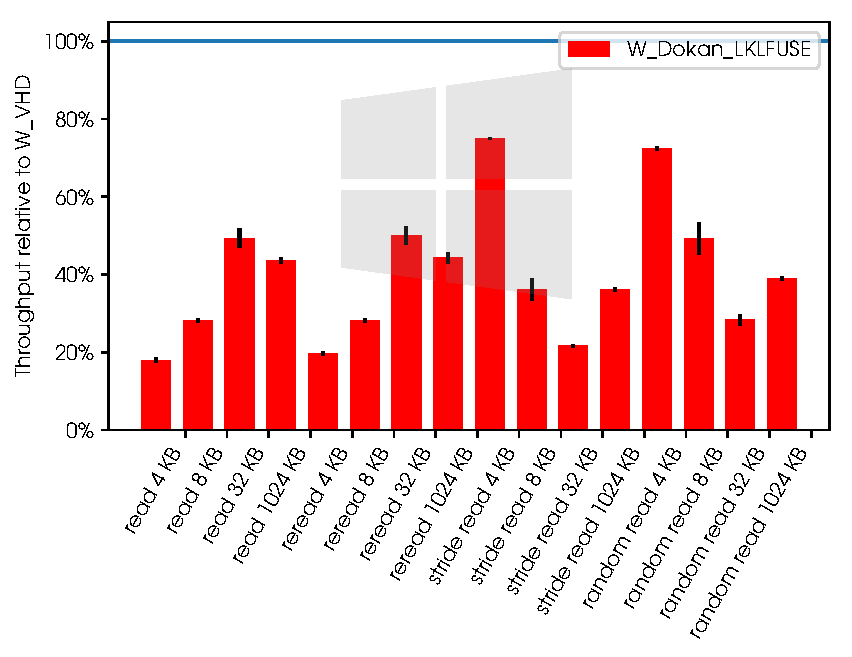
\includegraphics[page=1,width=0.87\paperwidth]{frames/img/relative_performance_filter_read_baseline_W_VHD_variants_W_Dokan_LKLFUSE}}
    \note{
        \begin{itemize}
            \item LKLFUSE-Dokan does worse in relative (and absolute) under Windows than under Linux.
            \item 40\% on average read performance. in opposite to Linux, higher blocksizes help, no readahead
            \item Dokan has several problems (no caching, fixed number of worker threads)
            \item interesting differences between blocksizes, not bigger is better. does not go through caching layer
            \item LKL maybe also has some room improvement, Windows API expert
        \end{itemize}
    }
\end{frame}

\begin{frame}[plain]
\frametitle{Throughput Relative to Windows VHD Mounting}
\vspace*{-1pt}
\makebox[\linewidth]{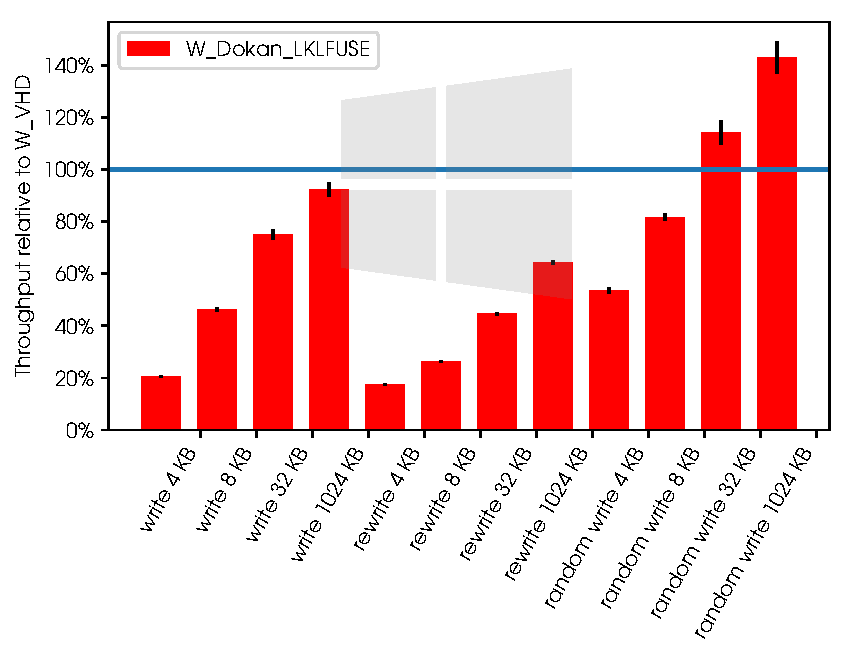
\includegraphics[page=1,width=0.87\paperwidth]{frames/img/relative_performance_filter_write_baseline_W_VHD_variants_W_Dokan_LKLFUSE}}
\note{
    \begin{itemize}
        \item write 65\%, in-line with read-workloads. Differences for different blocksizes
        \item also outperforming for random reads
    \end{itemize}
}
\end{frame}
